\section{Multivariate data analysis}

\subsection{Preprocessing}

\textbf{Missing data and Errors - } We inspect our dataset to find missing data (blanks\textbackslash Na's) or error values (e.g. negative numbers of rooms). Luckily our data is complete and we didn't need to handle and missing values.

\textbf{Outliers - } To determine if there are outliers on the data set, we will use the Robustified Mahalanobis distance  iterative algorithm (fig.\ref{mahalanobis}) from the Moutlier library function. To that purpose, we first filter out the categorical variables of the dataset and then feed the resulting data set into the algorithm. The results are the individuals sorted by their distance to the centroid. Our conlusion is that the first 8 individuals in that ordering are outliers. We remove them from the dataset.



\begin{figure}[H]
\minipage{0.5\textwidth}%
    \centering
        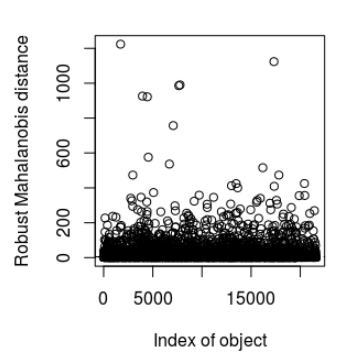
\includegraphics[width=0.7\textwidth]{img/mahalanobis.png}
    \caption{Robustified Mahalanobis distance for outliers detection }\label{mahalanobis}
\endminipage\hfill
\minipage{0.5\textwidth}%
    \centering
        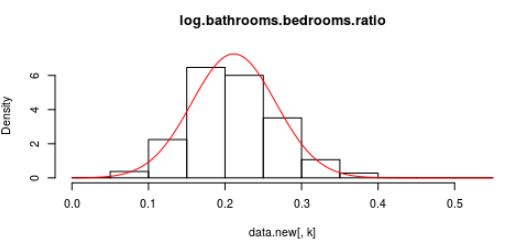
\includegraphics[width=0.9\textwidth]{img/gauss01.png}
    \caption{Plot of the histogram of a variable with a Normal distribution with same mean and variance }\label{gauss01}
\endminipage
\end{figure}
\vspace*{-15pt}

\subsection{Exploratory data analysis}
Briefly looking in the dataset's features (Table.\ref{table:dataFeatures}) we can see that not all features are useful for our work. We removed "id" and "date" from our table. The unique ID of individual is meaningless. Since we don't do time series analysis the date of sale is also useless. More details about feature extraction will be explained later.

\textbf{Histograms}

We start by ploting histograms of different variables of the dataset. With those we can start to estimate if data is far from normally distributed, if variables are from one or more than one process(fig.\ref{gauss01}).





\textbf{Plots}

We can also plot variables of the dataset by pairs, in order to appreciate which variables seem to be more correlated. 
We start by ploting variables with respect of the target (house price).

\begin{figure}[H]
    \centering
        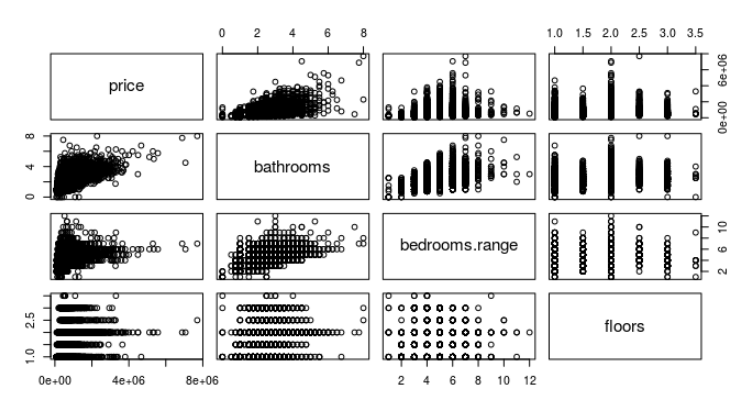
\includegraphics[width=0.8\textwidth]{img/pairs01.png}
    \caption{Plot of different variables against the price }\label{fig:rf_sfs}
\end{figure}

We expect to have some correlation based on the plots.

\textbf{Logarithm and ratio transformations}

We also explored how applying a logarithm to a variable or creating a ratio between 2 variables would affect the apparent correlation of the new variable with the target (house price):
\begin{figure}[H]
    \centering
        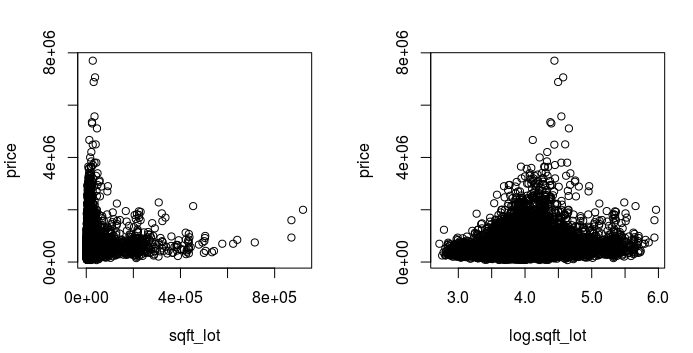
\includegraphics[width=0.8\textwidth]{img/log02.png}
    \caption{Plot the effect of the logarithm transformation }\label{fig:rf_sfs}
\end{figure}

We then decided to create some features that contain those transformations. (See section 3)

\textbf{Gaussianization}

It is important to know if the variables of the dataset are far or close to normality, in order to use some models that depend on the normality assumption(fig.\ref{gauss01}).

This is just approximate, but in case we find variables that deviate a from normality we can try to transform variables into a Gaussian version using the Box-Cox transform.

\begin{figure}[H]
    \centering
        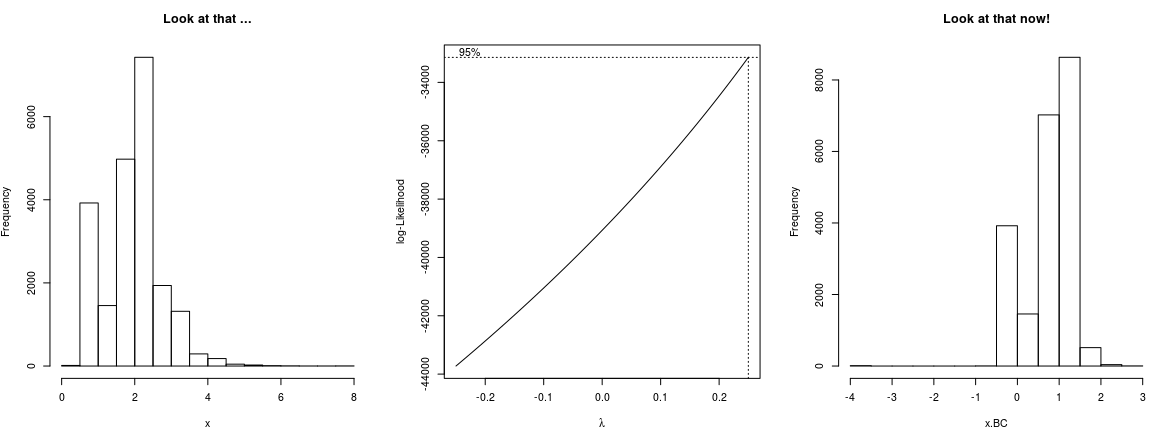
\includegraphics[width=0.8\textwidth]{img/Gauss03.png}
    \caption{Box-Cox transform for Gaussianization of a variable }\label{fig:rf_sfs}
\end{figure}

After trying some of those, it does not seem possible to Guassianize the variables of this dataset.


\subsection{Unsupervised analysis}


\begin{multicols}{2}

\textbf{PCA} In order to find some structure in the data we run PCA, as we can see in Figure.\ref{fig:PCA} there are strong correlation with many of the variable in the data set to our target (price variable). We learn that the area of living, the grade given by the city and number of bedrooms and bathrooms are important to when we want to analyze the price. On the other hand, the size of the basement and the properly size are not that important. 

\begin{figure}[H]
\centering
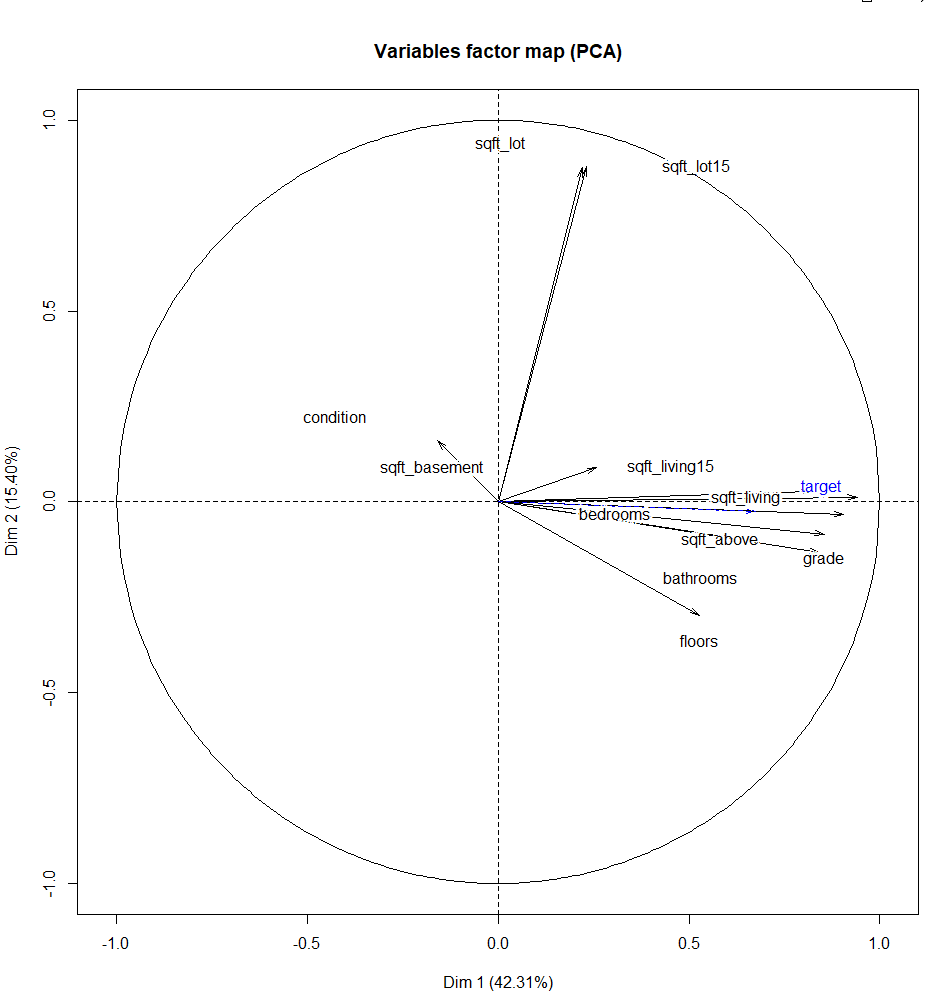
\includegraphics[width=0.49\textwidth]{img/PCA.png}
\caption{PCA}
\label{fig:PCA}
\end{figure}

\textbf{Clustering}
We clustered the individuals using hierarchical clustering. We did it using only continuous variables in order to see if we have some pattern in the data. As we can see in Fig.\ref{fig:hcluster}, more than $85\%$ of the individuals are grouped in a single cluster, the rest are divided into 2-3 clusters with smaller size. therefore, we deduce that we will not split our data into cluster and we will explore it as a whole.
% In case we will have time we would like to write something about the clustring using the projected individuals using PCA.
\begin{figure}[H]
\centering
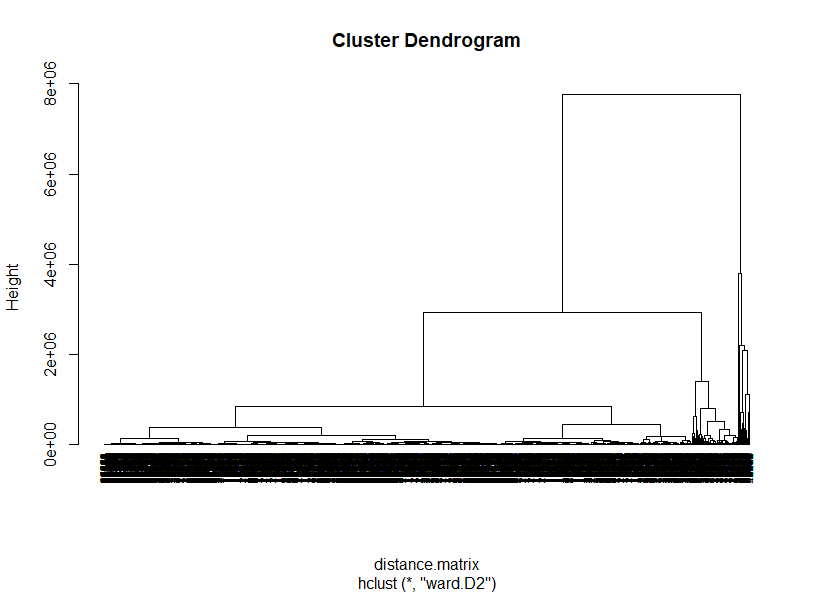
\includegraphics[width=0.48\textwidth]{img/Hclustering.png}
\caption{Hierarchical Clustering}
\label{fig:hcluster}
\end{figure}
\end{multicols}



